\chapter{Countermeasures Implementations}
\chaptermark{Countermeasures Implementations}
\label{chapter:countermeasures}
\minitoc

%%%%%%%%%%%%%%%%%%%%%%%%%%%%%%%%%%%%%%%%%%%%%%%%%%%%%%%%%%%%%%%%%%%%%%%%%%%%%%%%%%%%%%%%%%%%%%%
\section{Introduction}
Previous chapters have shown that the D-RI5CY's DIFT security mechanism is vulnerable to FIAs, mainly due to single-bit flips. This D-RI5CY essentially uses single-bit registers, as its data path is a single bit.

In this chapter, we present two countermeasures in order to protect the DIFT against fault injection attacks, and bit-flip.
The first countermeasure implemented to detect and prevent the use of corrupted data is simple parity. We selected the simple parity code as the error detection countermeasure because of its suitability and limited overhead.
The second countermeasure is implemented to detect any single-bit errors that may occur, but also to correct them without time overhead. With this countermeasure, we want to correct to the nearest cycle so that the fault cannot propagate and give a potential attacker the impression that the fault he injected had no effect on the system.
This work has been published in ISVLSI 2024~\cite{PRLG-24-isvlsi}.

The first section of this chapter presents the different fault models considered. Then, the second section details the implementation of simple parity and briefly presents how it works. Afterwards, the third section presents the working of Hamming code, with a simple example, and details our implementation. Finally, we discuss these countermeasures and compare them.

%%%%%%%%%%%%%%%%%%%%%%%%%%%%%%%%%%%%%%%%%%%%%%%%%%%%%%%%%%%%%%%%%%%%%%%%%%%%%%%%%%%%%%%%%%%%%%%
\section{Fault models used in this chapter}
In Chapter~\ref{chapter:dift_assessment}, we assessed the design by considering \textit{single bit-flip in one register at a given clock cycle}, \textit{set to 0}, and \textit{set to 1} fault models. The conclusion of this chapter was that the D-RI5CY is vulnerable to single bit-flip.

In this chapter, we consider an attacker able to inject faults into DIFT-related registers, leading to single bit-flips at any position of the targeted register. To reach this objective, any DIFT-related register maintaining 1-bit tag value, driving the tag propagation or the tag update process or maintaining the security policy configuration can be targeted. Studies presented in~\cite{ZDCRT-12-dcis,CLFT-14-cosade} have shown that such precise single bit-flip attacks targeting registers can be performed using, for example, laser shots. We also consider an attacker able to inject a single bit-flip in two registers at two distinct clock cycles, with a minimum delay of one clock cycle.

%%%%%%%%%%%%%%%%%%%%%%%%%%%%%%%%%%%%%%%%%%%%%%%%%%%%%%%%%%%%%%%%%%%%%%%%%%%%%%%%%%%%%%%%%%%%%%%
\section{Countermeasure 1: Simple Parity}
\label{chapter:simpleparity}

Error detection is often achieved through the use of parity codes, which involve adding an extra bit to the data bits for redundancy. Simple parity codes can detect single-bit errors. Simple parity can take into account odd parity or even parity, which means in case of an even parity, the number of bit set to '\texttt{1}' will be even with the message bits and parity bit.

%%%%%%%%%%%%%%%%%%%%%%%%%%%%%%
\subsection{Presentation of the simple parity}
Simple parity involves adding one bit to the data. This one bit store the parity of the initial message. Figures~\ref{fig:simpleparity_functionning} shows how to data and the parity bit are combined. The data, in blue, and the parity bit, in red, are associated to form an encoded data.

\begin{figure}[ht]
    \centering
    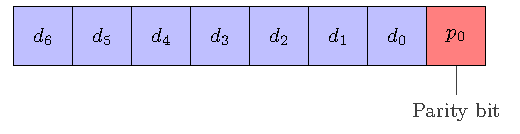
\includegraphics[page=1]{c5_countermeasures_dift/img/simple_parity.pdf}
    \caption{Simple Parity - functioning}
    \label{fig:simpleparity_functionning}
\end{figure}

Equation~\ref{equat:simpleparity} shows how the parity bit is computed. Each bit of the initial message is xor'd to show parity. Table~\ref{tab:xor_truthtable} present the truth table of XOR operations.

\begin{equation} \label{equat:simpleparity}
    \begin{split}
        p_{0} &= d_{0} \oplus d_{1} \oplus d_{2} \oplus d_{3} \oplus d_{4} \oplus d_{5} \oplus d_{6}
    \end{split}
\end{equation}

\begin{table}[t]
    \centering
    \caption{XOR truth table}
    \label{tab:xor_truthtable}
    \begin{tabular}{@{}c|c|c@{}}
        \toprule
        A & B & $A \oplus B$ \\\midrule
        0 & 0 & 0            \\
        0 & 1 & 1            \\
        1 & 0 & 1            \\
        1 & 1 & 0            \\
        \bottomrule
    \end{tabular}
\end{table}

Figures~\ref{fig:simpleparity_example_1} and \ref{fig:simpleparity_example_2} show an example of a message with its parity bit associated. The message is \texttt{0b1001101} in binary, then, as there is an even number of '\texttt{1}', the parity bit is set to '\texttt{0}' (cf Table~\ref{tab:xor_truthtable}).
\begin{figure}[ht]
    \centering
    \begin{subfigure}[b]{0.49\textwidth}
        \includegraphics[width=\textwidth, page=2]{c5_countermeasures_dift/img/simple_parity.pdf}
        \caption{Initial message}
        \label{fig:simpleparity_example_1}
    \end{subfigure}
    \hfill
    \begin{subfigure}[b]{0.49\textwidth}
        \includegraphics[width=\textwidth, page=3]{c5_countermeasures_dift/img/simple_parity.pdf}
        \caption{Message with its parity bit}
        \label{fig:simpleparity_example_2}
    \end{subfigure}
    \hfill
    \begin{subfigure}[b]{0.49\textwidth}
        \includegraphics[width=\textwidth, page=4]{c5_countermeasures_dift/img/simple_parity.pdf}
        \caption{Single-bit fault inside the message}
        \label{fig:simpleparity_faulted_example_3}
    \end{subfigure}
    \hfill
    \begin{subfigure}[b]{0.49\textwidth}
        \includegraphics[width=\textwidth, page=5]{c5_countermeasures_dift/img/simple_parity.pdf}
        \caption{Two single-bit faults inside the message}
        \label{fig:simpleparity_faulted_example_4}
    \end{subfigure}
    \caption{Exemple of a simple parity computation}
    \label{fig:simpleparity_example}
\end{figure}

Figures~\ref{fig:simpleparity_faulted_example_3} and \ref{fig:simpleparity_faulted_example_4} present, respectively, two examples of when a fault occur or when two faults happen. In the first example, Figure~\ref{fig:simpleparity_faulted_example_3}, the bit $d_2$ is faulted.
As the faulted message is \texttt{0b1001001}, it means that the parity bit will change from \texttt{0} to \texttt{1}. Hence, the fault will be detected as the parity bit differs from original computed message (Figure~\ref{fig:simpleparity_example_2}).

In the second case, two faults happen in the message at bit $d_2$ and $d_5$. Hence, the faulted message will be \texttt{0b1101001}, so when the parity is computed, the parity bit will not change as there is still an even number of \texttt{1} compared to the initial message.

%%%%%%%%%%%%%%%%%%%%%%%%%%%%%%
\subsection{Implementation: Optimisation of redundancy bits}

\begin{table}[t]
    \centering
    \caption{DIFT-related protected registers - simple parity}
    \label{tab:sp_group}
    \begin{tabular}{@{}cccc@{}}
        \toprule
                & Protected register                                                                                & Number of protected bits & \begin{tabular}[c]{@{}c@{}}Number of parity\\ bits for Simple Parity\end{tabular} \\ \midrule
        Group 1 & TCR                                                                                               & 22                       & 1                                                                                 \\
        Group 2 & TPR                                                                                               & 22                       & 1                                                                                 \\
        Group 3 & Register File (Tag)                                                                               & 32                       & 1                                                                                 \\
        Group 4 & Tag destination address                                                                           & 5                        & 1                                                                                 \\
        Group 5 & \begin{tabular}[c]{@{}c@{}}16×1-bit registers\\ 3×2-bit registers\\ 1×4-bit register\end{tabular} & 26                       & 1                                                                                 \\ \midrule
        Total   &                                                                                                   & 107                      & 5                                                                                 \\
        \bottomrule
    \end{tabular}
\end{table}

\begin{figure}[ht]
    \centering
    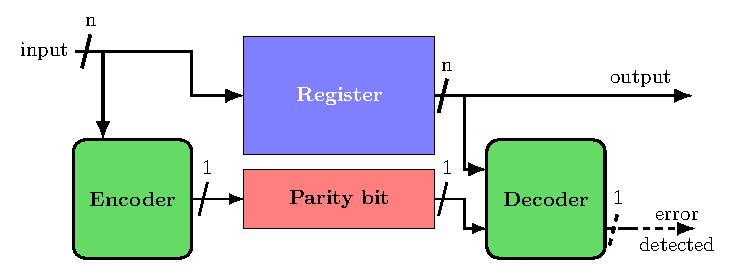
\includegraphics[page=1]{c5_countermeasures_dift/img/archi_contremesures.pdf}
    \caption{Implementation of simple parity}
    \label{fig:implementation_sp}
\end{figure}


%%%%%%%%%%%%%%%%%%%%%%%%%%%%%%%%%%%%%%%%%%%%%%%%%%%%%%%%%%%%%%%%%%%%%%%%%%%%%%%%%%%%%%%%%%%%%%%
\section{Countermeasure 2: Hamming Code}
\label{chapter:hammingcode}

%%%%%%%%%%%%%%%%%%%%%%%%%%%%%%
\subsection{Presentation of Hamming Code}

\begin{figure}[ht]
    \centering
    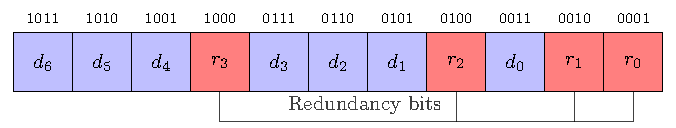
\includegraphics[page=1]{c5_countermeasures_dift/img/hamming_bit.pdf}
    \caption{Hamming code - functioning}
    \label{fig:hamming_functionning}
\end{figure}

\begin{equation} \label{equat:hamming_encoder}
    \begin{split}
        r_{0} &= d_{0} \oplus d_{1} \oplus d_{3} \oplus d_{4} \oplus d_{6} \\
        r_{1} &= d_{0} \oplus d_{2} \oplus d_{3} \oplus d_{5} \oplus d_{6} \\
        r_{2} &= d_{1} \oplus d_{2} \oplus d_{3} \\
        r_{3} &= d_{4} \oplus d_{5} \oplus d_{6}
    \end{split}
\end{equation}

%%%%%%%%%%%%%%%%%%%%%%%%%%%%%%
\subsection{Implementation 1: Optimisation of redundancy bits}

\begin{table}[t]
    \centering
    \caption{DIFT-related protected registers - Hamming code}
    \label{tab:hammingcode_group}
    \begin{tabular}{@{}cccc@{}}
        \toprule
                & Protected register                                                                                & Number of protected bits & \begin{tabular}[c]{@{}c@{}}Number of redundancy\\ bits for Hamming Code\end{tabular} \\ \midrule
        Group 1 & TCR                                                                                               & 22                       & 5                                                                                    \\
        Group 2 & TPR                                                                                               & 22                       & 5                                                                                    \\
        Group 3 & Register File (Tag)                                                                               & 32                       & 6                                                                                    \\
        Group 4 & Tag destination address                                                                           & 5                        & 4                                                                                    \\
        Group 5 & \begin{tabular}[c]{@{}c@{}}16×1-bit registers\\ 3×2-bit registers\\ 1×4-bit register\end{tabular} & 26                       & 5                                                                                    \\ \midrule
        Total   &                                                                                                   & 107                      & 25                                                                                   \\
        \bottomrule
    \end{tabular}
\end{table}

\begin{figure}[ht]
    \centering
    \includegraphics[page=2, width=\textwidth]{c5_countermeasures_dift/img/archi_contremesures.pdf}
    \caption{Implementation of Hamming Code}
    \label{fig:implementation_hc_1}
\end{figure}

\begin{figure}[ht]
    \centering
    \includegraphics[page=3, width=\textwidth]{c5_countermeasures_dift/img/archi_contremesures.pdf}
    \caption{Implementation of Hamming Code - Register Tile Tag}
    \label{fig:implementation_hc_2}
\end{figure}

%%%%%%%%%%%%%%%%%%%%%%%%%%%%%%%%%%%%%%%%%%%%%%%%%%%%%%%%%%%%%%%%%%%%%%%%%%%%%%%%%%%%%%%%%%%%%%%
\section{Discussion}

%%%%%%%%%%%%%%%%%%%%%%%%%%%%%%%%%%%%%%%%%%%%%%%%%%%%%%%%%%%%%%%%%%%%%%%%%%%%%%%%%%%%%%%%%%%%%%%
\section{Summary}

%%%%%%%%%%%%%%%%%%%%%%%%%%%%%%%%%%%%%%%%%%%%%%%%%%%%%%%%%%%%%%%%%%%%%%%%%%%%%%%%%%%%%%%%%%%%%%%